% ============================================================
% fig - ancilla layouts.tex
% Terminal postselection, one-ancilla and two-ancilla (conventional-site)
% check layouts on the conventional surface-code grid. The drawing is a
% standalone TikZ figure (paper-rework/layout-figure/ancilla-layouts.tex),
% compiled to figures/ancilla-layouts.pdf; the caption body lives here.
% ============================================================
\begin{figure}[!tb]
  \centering
  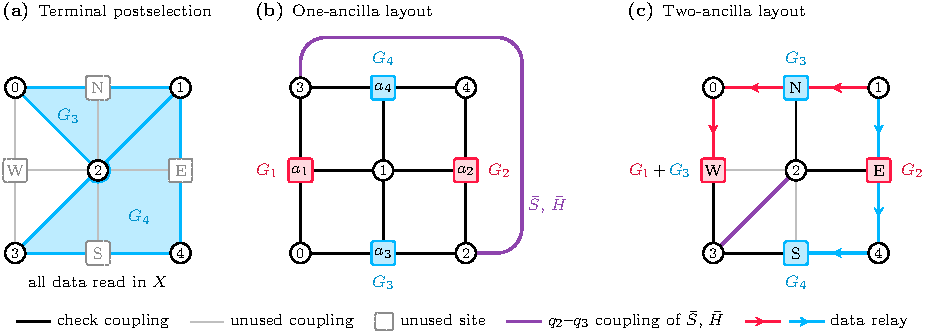
\includegraphics{figures/ancilla-layouts.pdf}% drawn at final size
  \caption{Stabilizer checks of the $[[5,1,2]]_3$ code on the conventional surface-code grid of data qutrits (circles) and ancilla sites (squares). Black and arrowed lines are couplings used by the check rounds; gray lines and dashed squares are unused. Red marks the $Z$-type $G_1$, $G_2$ and blue the $X$-type $G_3$, $G_4$. Purple lines mark the $q_2$--$q_3$ coupling of $CZ_{2\to3}$ in $\bar S$ and $\mathrm{SWAP}_{2,3}$ in $\bar H$. The label beside a site is its one readout per check round, modulo three and up to the syndromes' signs.
(a)~On the patch of \autoref{fig: 5-qutrit-code}, with $q_2$ at the center, terminal postselection uses no ancillas. The final $X$-basis readout of all data, with outcomes $x_j$, gives $G_3$, $G_4$ (shaded) and the logical outcome $x_0 + x_3$, not $G_1$ or $G_2$.
(b)~With $q_1$ at the center, ancilla $a_j$ neighbors all three data qutrits of $G_j$, but $q_2$ and $q_3$ sit at opposite corners and need a long-range coupling.
(c)~With $q_2$ at the center, $q_2$ and $q_3$ are diagonal neighbors, but $G_1$ and $G_4$ contain the opposite corners $q_1$ and $q_3$ and need two sites each. Arrows trace the data relay of their $q_1$ parts (\autoref{tab:conv_round}). N, holding $G_3$, collects the $q_1$ part of $G_1$ and lends its value to $q_0$, where W collects it with the rest of $G_1$, so W reads $G_1$ shifted by $G_3$. N then takes the value back and clears its $q_1$ part. E relays the $q_1$ part of $G_4$ likewise, through $q_4$ to S in the $X$ basis, before measuring $G_2$. All four readouts vanish exactly when all four syndromes do.}
  \label{fig:ancilla_layouts}
\end{figure}
